%==============================================================================
% presentation.tex
%==============================================================================


%==============================================================================
% Configuration
%==============================================================================

% Internationalisation
\usepackage[utf8]{inputenc}
\usepackage[T1]{fontenc}
% \usepackage[ngerman]{babel}

% Different packages
\usepackage{url}
\usepackage{color,listings,paralist}
\usepackage{enumerate}
\usepackage{tabularx}
\usepackage{alltt}

% Use default Acrobat reader fonts
\usepackage{mathpazo}

% Use CM fonts (increases document size)
\usepackage{ae}

% Use images
\usepackage{graphicx}

% Configure beamer
\usetheme[secheader]{Ikhono}
\usefonttheme[onlylarge]{structurebold}
\setbeamertemplate{navigation symbols}{}

% Variables
\providecommand{\Title}{Mining Software Repositories for Intelligent
  Software Maintenance}
\providecommand{\ShortTitle}{Mining software repositories}
\providecommand{\Author}{Thomas Weibel <weibelt@ethz.ch>}
\providecommand{\Institute}{SETLabs, Infosys Tech. Ltd., Bangalore}
\providecommand{\Date}{December 1, 2009}

% PDF settings
\hypersetup{
  pdftitle={\Title},
  pdfauthor={\Author},
  pdfsubject={\Institute},
  pdfkeywords={software engineering, portable, efficient, parallel
    programming language} 
}

% Titlepage
\title[\ShortTitle]{\Title}
\author{\Author}
\institute{\Institute}
\date{\Date}

% Listings
\lstdefinelanguage[]{Metrics}[]{}{
  keywords={if,then,else,end}
}
\lstdefinestyle{Default}{
  language=Metrics,
  tabsize=2,
  mathescape=true,
  inputencoding=utf8,
  showstringspaces=false,
  fontadjust=true,
  basicstyle=\ttfamily,
  keywordstyle=\color{blue}\bfseries,
}
\lstset{style=Default}


%==============================================================================
% Document
%==============================================================================

\begin{document}


% Titlepage
\begin{frame}[plain]
  \titlepage
\end{frame}

\note{
}


\section*{Introduction}

\begin{frame}{Executive Summary}
  \begin{itemize}
  \item Change management with version control systems
  \item Improving software maintenance through software repository
    mining
  \item Framework for preventive maintenance
  \item Metrics for localization
  \item Study of Open Source projects
  \end{itemize}
\end{frame}

\note{
}


\section{Version Control}

\begin{frame}{Outline}
  \tableofcontents[current]
\end{frame}

\note{
}

\begin{frame}{Version Control}
  \begin{center}
    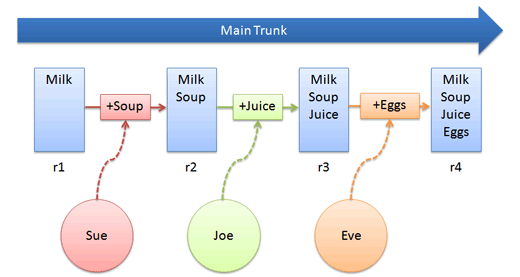
\includegraphics[scale=0.35]{figures/vcs}
  \end{center}

  \vspace{\stretch{1}}

  \begin{itemize}
  \item Management of changes to computer files in a repository
  \item Changes identified by a number or letter code (``revision'')
  \item Each revision associated with timestamp and person
    making the change
  \item Version control systems: CVS, Subversion, Git, ...
  \end{itemize}
\end{frame}

\note{
  \begin{itemize}
  \item Version control is the management of changes to documents,
    programs, and other information stored as computer files. It is
    most commonly used in software development, where a team of people
    may be changing the same files.
  \item Changes are usually identified by a number or letter code,
    termed the ``revision''. For example, an initial set of files is
    ``revision 1''. When the first change is made, the resulting set
    is ``revision 2'', and so on.
  \item Each revision is associated with a timestamp and the person
    making the change.
  \end{itemize}
}

\begin{frame}[containsverbatim]{Working Copy, Commits and Change Sets}
  \begin{itemize}
  \item Working copy: Local copy of files from a repository
  \item Commit: Writing changes to the working copy into the
    repository
  \item Change set: Set of changes made in a single commit
  \end{itemize}

  \vspace{\stretch{1}}

\begin{verbatim}
  commit 3d2d827f5ca5e32816194119d5c980c7e04474a6
  Author: Michael S. Tsirkin <mst@redhat.com>
  Date:   Mon Sep 21 17:03:51 2009 -0700

      mm: move use_mm/unuse_mm from aio.c to mm/

  M       fs/aio.c
  A       include/linux/mmu_context.h
  M       mm/Makefile
  A       mm/mmu_context.c
\end{verbatim}
\end{frame}

\note{
  \begin{itemize}
  \item The working copy is the local copy of files from a repository,
    at a specific time or revision.
  \item A commit occurs when a copy of the changes made to the working
    copy is written or merged into the repository.
  \item On version control systems with atomic multi-change commits, a
    change set identifies the set of changes made in a single commit.
  \end{itemize}
}


\section{Mining Software Repositories}

\begin{frame}{Outline}
  \tableofcontents[current]
\end{frame}

\note{
}

\begin{frame}{Software Repository Mining}
  \begin{columns}[c]
    \begin{column}{0.60\textwidth}
      \begin{itemize}
      \item Version control systems contain large amounts of
        historical information: ``\textit{Who} changed \textit{what},
        \textit{why} and \textit{when}.''
      \item Learn from the past to shape the future
      \item Automated extraction, collection, and abstraction of
        information from software development data
      \end{itemize}
    \end{column}
    \begin{column}{0.40\textwidth}
      
\includegraphics[width=\textwidth]{figures/mining}
    \end{column}
  \end{columns}
\end{frame}

\note{ 
  \begin{itemize}
  \item Version control systems contain large amounts of historical
    information that can give deep insight into the evolution of a
    software project: ``\textit{Who} changed \textit{what},
    \textit{why} and \textit{when}.''
  \item When mining software archives, we want to learn from the past
    to shape the future.
  \item The mining of software repositories is concerned with the
    automated extraction, collection, and abstraction of information
    from available software development data.
  \end{itemize}
}

\begin{frame}{Populating Version History Database}
  \begin{center}
    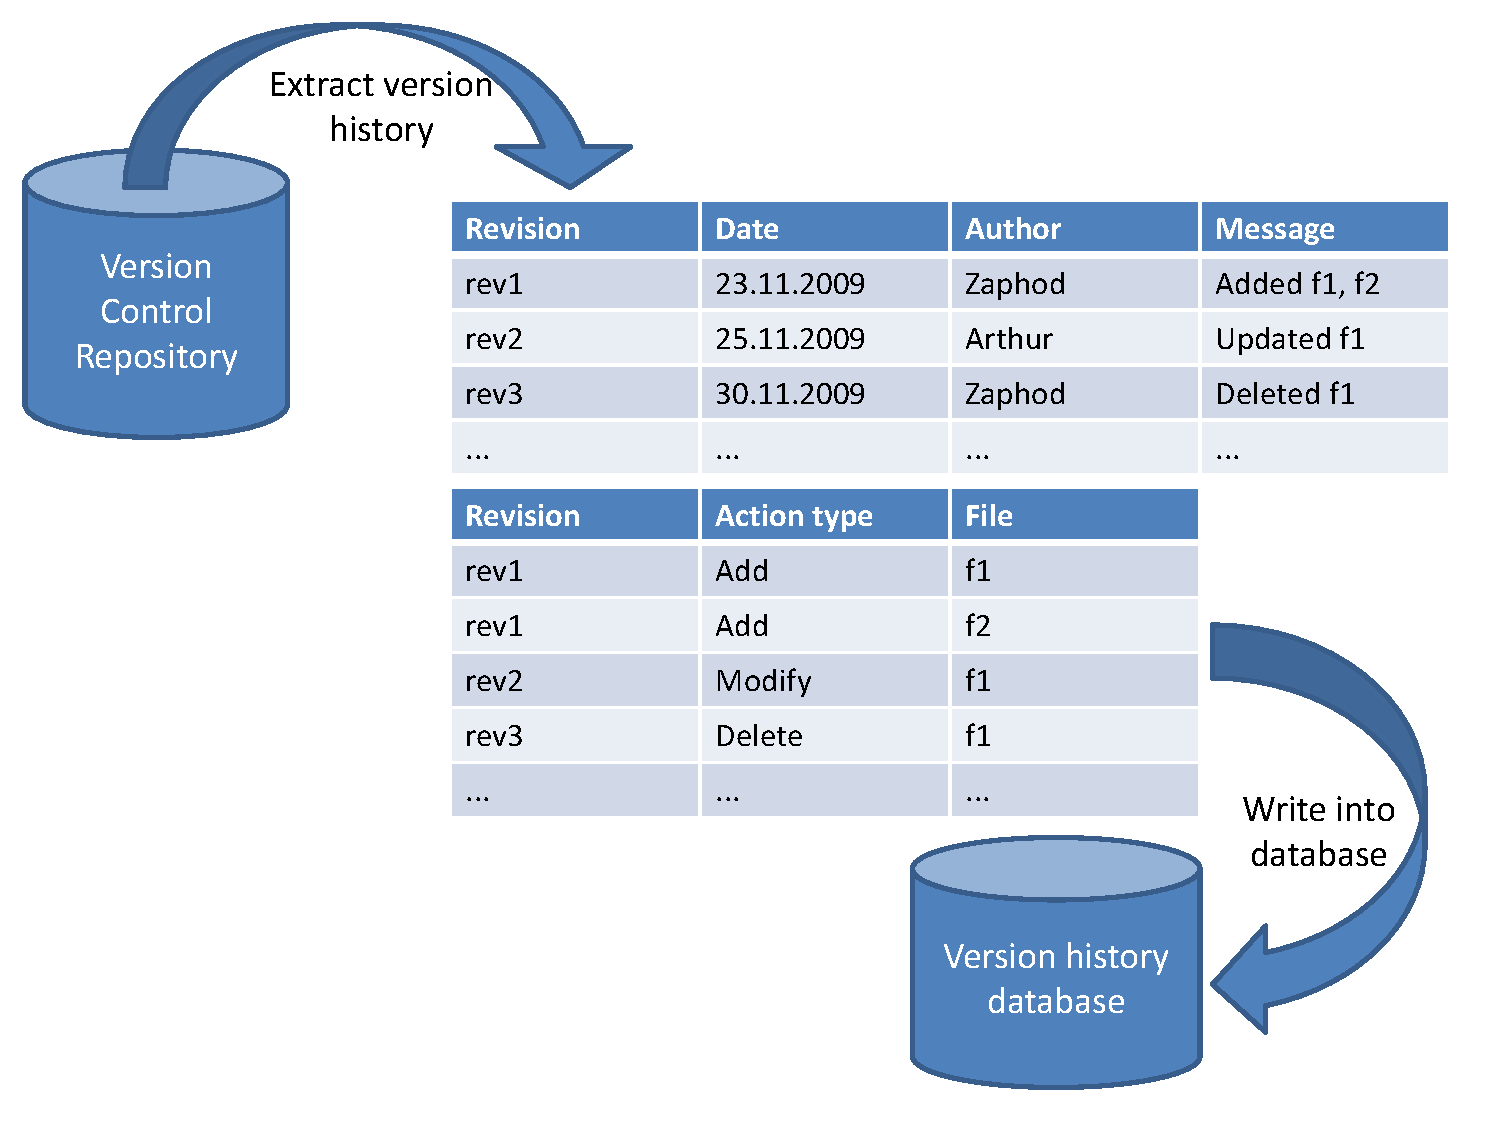
\includegraphics[width=0.95\textwidth]{figures/extracting-version-history}
  \end{center}
\end{frame}

\note{
}

\subsection{Frequent Item Set Mining}

\begin{frame}{Frequent Item Set Mining}
  \begin{columns}[c]
    \begin{column}{0.5\textwidth}
      \begin{itemize}
      \item Popular method for market basket analysis
      \item Identify sets of products frequently bought together
      \item Our framework applies frequent item set mining to the
        version history of software repositories
      \item Identify which code files have been frequently changed
        together
      \end{itemize}
    \end{column}
    \begin{column}{0.5\textwidth}
      \begin{center}
        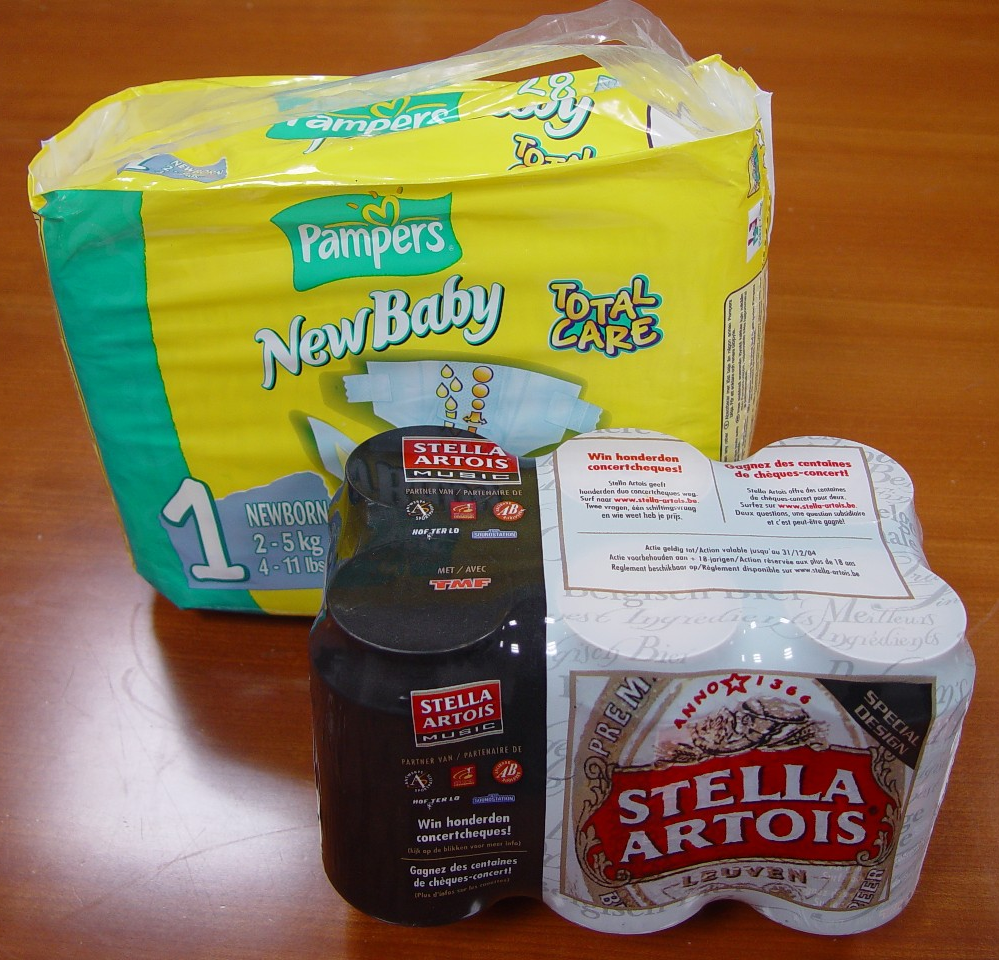
\includegraphics[width=\textwidth]{figures/frequent-item-set} \\
        \tiny{Source: \url{http://research.nii.ac.jp/~uno}}
      \end{center}
    \end{column}
  \end{columns}
\end{frame}

\note{
  \begin{itemize}
  \item Finding frequent item sets in a set of transactions is a
    popular method for so-called market basket analysis. It aims at
    finding regularities in the shopping behaviour of customers of
    supermarkets, mail-order companies, online-shops and so forth.
  \item In particular, it tries to identify sets of products that are
    frequently bought together.
  \item In our framework, we apply frequent item set mining to the
    version history of software repositories.
  \item The goal is to find out, which code files have been frequently
    changed together.
  \end{itemize}
}

\begin{frame}[containsverbatim]{Frequent Item Set Mining: Transactions}
  \begin{itemize}
  \item Transactions: Change sets
  \item Example:
\begin{verbatim}
  { fs/aio.c, include/linux/mmu_context.h, 
    mm/Makefile, mm/mmu_context.c }
\end{verbatim}
  \end{itemize}

  \vspace{\stretch{1}}

\begin{verbatim}
  commit 3d2d827f5ca5e32816194119d5c980c7e04474a6

  M       fs/aio.c
  A       include/linux/mmu_context.h
  M       mm/Makefile
  A       mm/mmu_context.c
\end{verbatim}
\end{frame}

\note{
  \begin{itemize}
  \item A change set identifies the set of changes made in a single
    commit to the version control system. We take change sets as our
    transactions in frequent item set mining.
  \item In the example below, the transaction consist of four files.
  \end{itemize}
}

\begin{frame}{Frequent Item Set Mining: Definitions}
  \begin{itemize}
  \item The \alert{transaction database} contains all change sets
  \item Members of transactions are called \alert{items}
  \item An \alert{item set} is a subset of possible items
  \item \alert{Support} of an item set $i$: sup($i$) $:=$ number of
    transactions $t$ that support (i.e. contain) $i$
  \end{itemize}
\end{frame}

\note{
}

\begin{frame}{Frequent Item Set Mining: Association Rules}
  \begin{center}
    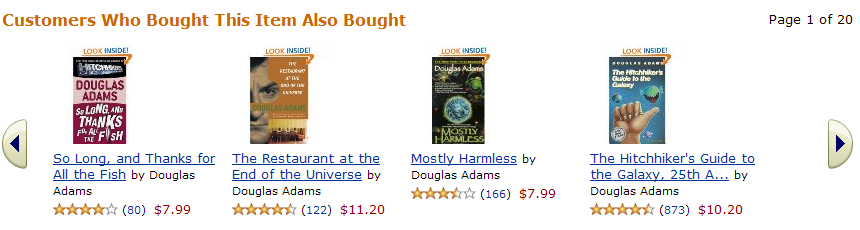
\includegraphics[width=\textwidth]{figures/frequent-items} \\
    \tiny{Source: \url{amazon.com}}
  \end{center}

  \vspace{\stretch{1}}

  \begin{itemize}
  \item \alert{If} a customer buys \alert{bread} and \alert{wine}, \\
    \alert{then} she will probably also buy \alert{cheese}
  \item Problem decomposed into two subproblems:
    \begin{itemize}
    \item Finding frequent item sets with minimum support
    \item Generate association rules with minimal confidence
    \end{itemize}
  \item Confidence for association rule $R: X \rightarrow Y$:
    $\text{conf}(R) = \text{conf}(X \rightarrow Y) =
    \text{sup}(X \cup Y)/\text{sup}(X)$
  \end{itemize}
\end{frame}

\note{
}

\begin{frame}{Frequent Item Set Mining: Example}
  \begin{center}
    \begin{tabular}{c|l}
      Transaction IDs & Transactions (Files) \\ \hline \hline
      1 & $\{1, 2, 3, 4\}$ \\ \hline
      2 & $\{2, 3, 4\}$ \\ \hline
      3 & $\{2, 3\}$ \\ \hline
      4 & $\{1, 2, 4\}$ \\ \hline
      5 & $\{1, 2, 3, 4\}$ \\ \hline
      6 & $\{2, 4\}$ \\
    \end{tabular}
  \end{center}
\end{frame}

\note{
}

\subsection{Maintenance Challenges}

\begin{frame}{Maintenance Challenges}
  \begin{itemize}
  \item Predicting Faults
  \item Improve Bug Finding Techniques
  \item Predicting Changes
  \item Code Ownership
  \item Traceability Links
  \item Understanding Software Evolution
  \end{itemize}

  \vspace{\stretch{1}}

  \begin{center}
    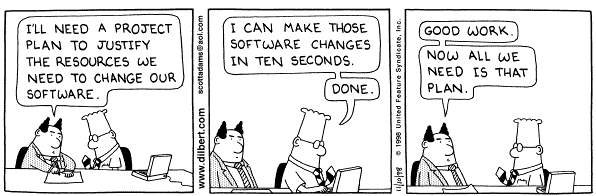
\includegraphics[width=0.7\textwidth]{figures/dilbert-software-changes}
  \end{center}
\end{frame}

\note{
}

\begin{frame}{Predicting Faults}
  TODO
\end{frame}

\note{
}

\begin{frame}{Improve Bug Finding Techniques}
  TODO
\end{frame}

\note{
}

\begin{frame}{Predicting Changes}
  TODO
\end{frame}

\note{
}

\begin{frame}{Code Ownership}
  TODO
\end{frame}

\note{
}

\begin{frame}{Traceability Links}
  TODO
\end{frame}

\note{
}

\begin{frame}{Understanding Software Evolution}
  TODO
\end{frame}

\note{
}


\section{Framework}

\begin{frame}{Outline}
  \tableofcontents[current]
\end{frame}

\note{
}

\begin{frame}{Architecture}
  \begin{center}
    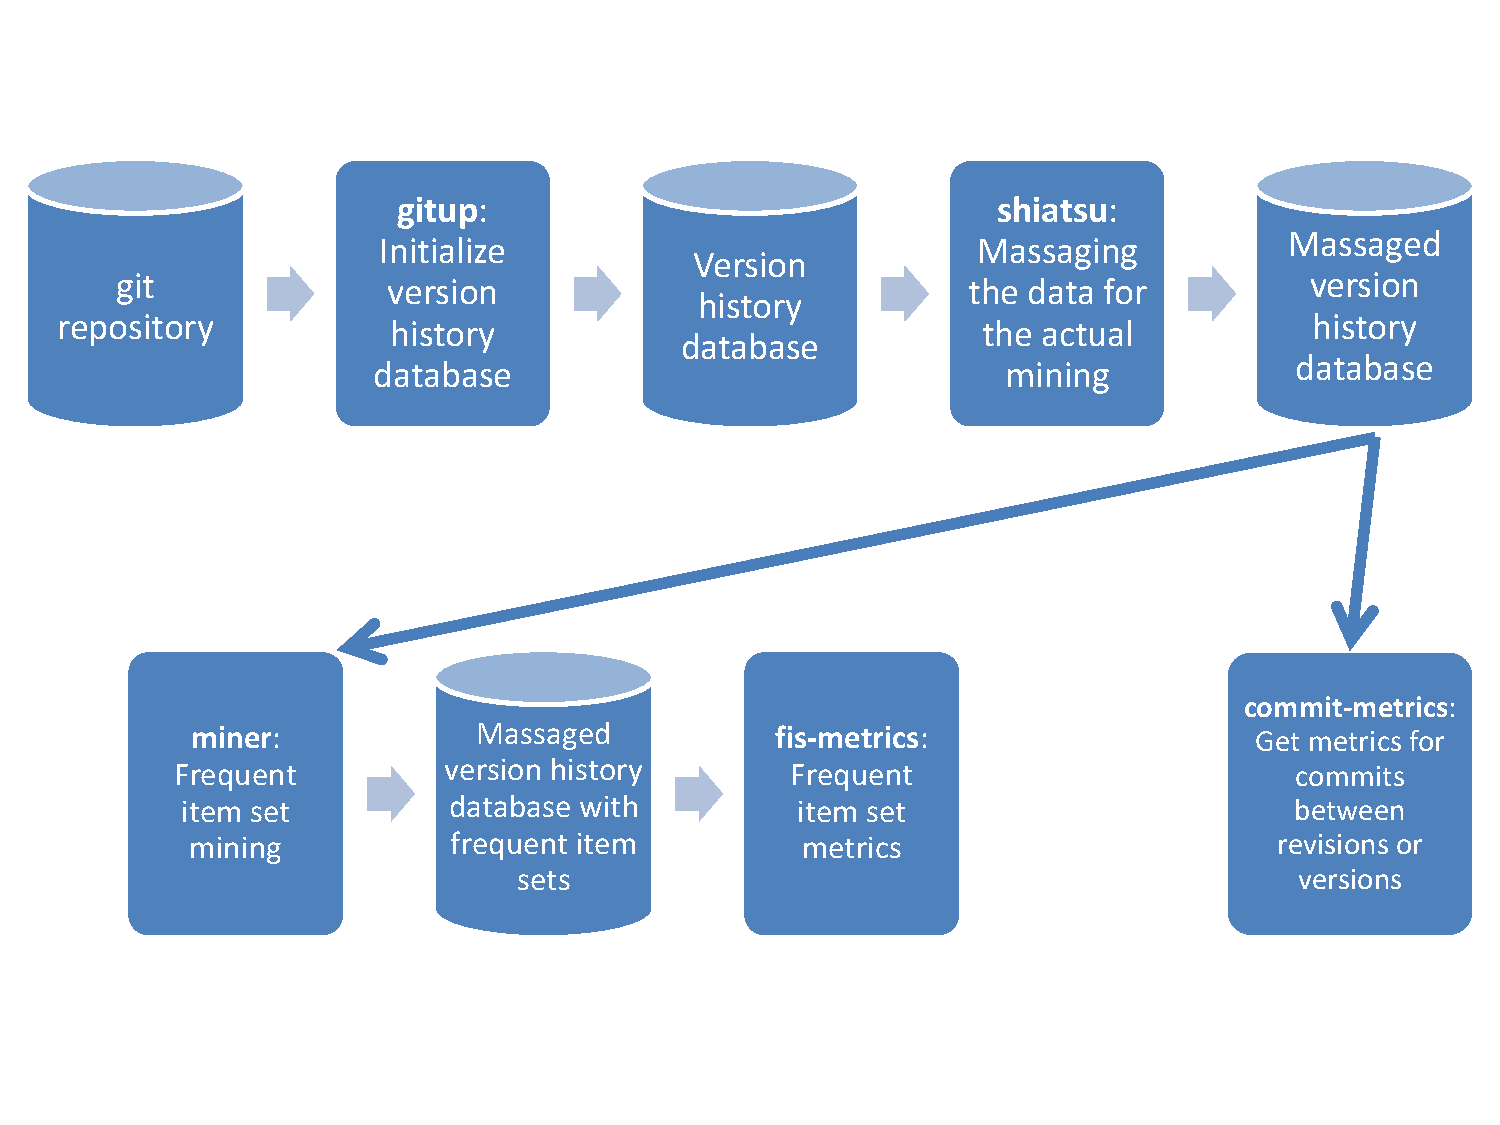
\includegraphics[width=0.95\textwidth]{figures/miner-architecture}
  \end{center}
\end{frame}

\note{
}

\begin{frame}{Git}
  \begin{itemize}
  \item Free distributed version control system
  \item Initially designed and developed for Linux kernel development
  \item Every Git working directory is a full-fledged repository:
    \begin{itemize}
    \item Complete history
    \item Full revision tracking capabilities
    \item Not dependent on network access or a central server
    \end{itemize}
  \item Repositories of other version control systems like Subversion
    can easily be converted into Git repositories
  \item Only need to write mining and analysis tools for one format
    rather than many
  \end{itemize}
\end{frame}

\note{
  \begin{itemize}
  \item Git is a free distributed version control system.
  \item It was initially designed and developed by Linus Torvalds for
    Linux kernel development.
  \item Every Git working directory is a full-fledged repository with
    complete history and full revision tracking capabilities, not
    dependent on network access or a central server.
  \item Repositories of other version control systems like CVS or
    Subversion can easily be converted into Git repositories.
  \item This means we only need to write mining and analysis tools for
    one format rather than many.
  \end{itemize}
}

\begin{frame}{Populating the Version History Database}
  \begin{itemize}
  \item Gitup generates logfile and initializes versions history
    database
  \item Shiatsu massages the data to be used by the metrics
    applications
    \begin{itemize}
    \item Set modularization according to specified directory depth
    \item Remove deleted files
    \item Set number of modifications
    \item Heuristics for file moves
    \end{itemize}
  \end{itemize}

  \vspace{\stretch{1}}

  \begin{center}
    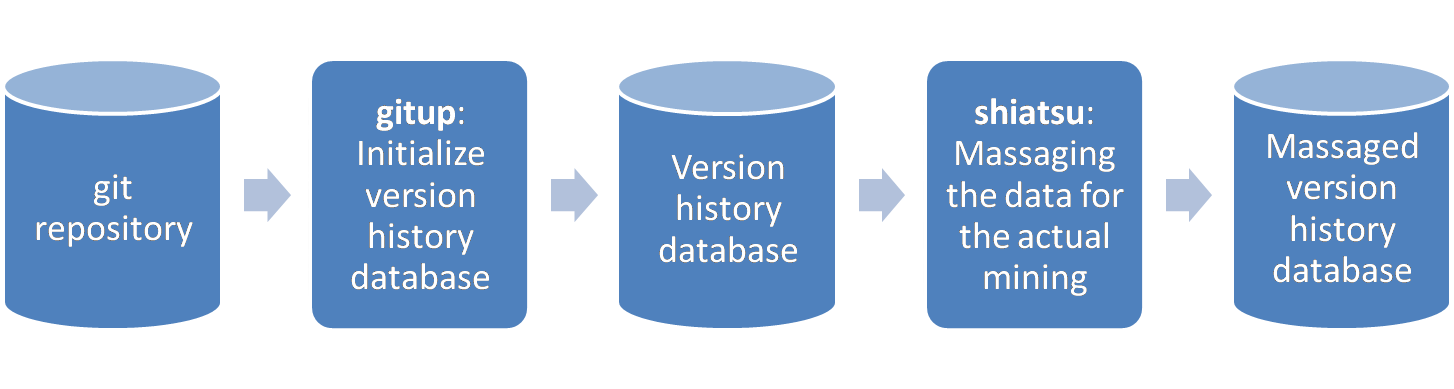
\includegraphics[width=0.95\textwidth]{figures/initialize-database}
  \end{center}
\end{frame}

\note{
}


\section{Novelty}

\begin{frame}{Outline}
  \tableofcontents[current]
\end{frame}

\note{
}

\begin{frame}{Change Localization}
  \begin{itemize}
  \item A change is well localized, if it touches only one or very few
    modules
  \item A change is not well localized, if it touches many modules
  \item Apply change localization for frequent item sets
  \end{itemize}

  \vspace{\stretch{1}}

  \begin{block}{Hypothesis}
    Changes in frequent item sets in well modularized software systems
    are localized
  \end{block}
\end{frame}

\note{
}

\begin{frame}[containsverbatim]{Change Localization: Example}
  \begin{itemize}
  \item Well localized: Touches only one module
\begin{verbatim}
  dlls/ntdll/signal_i386.c
  dlls/ntdll/thread.c
\end{verbatim}
  \item Badly localized: Touches four modules out of five possible
\begin{verbatim}
  if1632/thunk.c
  include/process.h
  loader/task.c
  scheduler/process.c
  scheduler/thread.c
\end{verbatim}
  \item Not localized at all: Touches all possible modules
\begin{verbatim}
  files/dos_fs.c
  scheduler/syslevel.c
  tools/winapi-check  
\end{verbatim}
  \end{itemize}
\end{frame}

\note{
}

\begin{frame}{Change Localization Metrics}
  \begin{itemize}
  \item Value between $0$ and $1$
  \item $0$: Not localized at all
  \item $1$: Fully localized
  \end{itemize}

  \vspace{\stretch{1}}

  \[
  \underline{\sum_{i = \text{FIS}_1}^{\text{FIS}_n} 1 -
    \left(\text{if}\left( i.\text{modules\_touched} == 1, 0,
        \frac{i.\text{modules\_touched}}{i.\text{files\_touched}}
      \right) \right)}
  \]
  \[
  n
  \]
\end{frame}

\note{
}


\section{Experiments}

\begin{frame}{Outline}
  \tableofcontents[current]
\end{frame}

\note{
}

\subsection{Linux 2.6}

\begin{frame}{Linux 2.6}
  \begin{columns}[c]
    \begin{column}{0.60\textwidth}
      \begin{itemize}
      \item Unix-like operating system kernel
      \item Repository checked out on November 19, 2009
      \item $25,277$ code files
      \item $168,800$ commits
      \end{itemize}
    \end{column}
    \begin{column}{0.40\textwidth}
      
\includegraphics[width=\textwidth]{figures/linux-logo}
    \end{column}
  \end{columns}
\end{frame}

\note{
}

\begin{frame}{Linux 2.6: Frequent Item Set Metrics}
  \begin{center}
    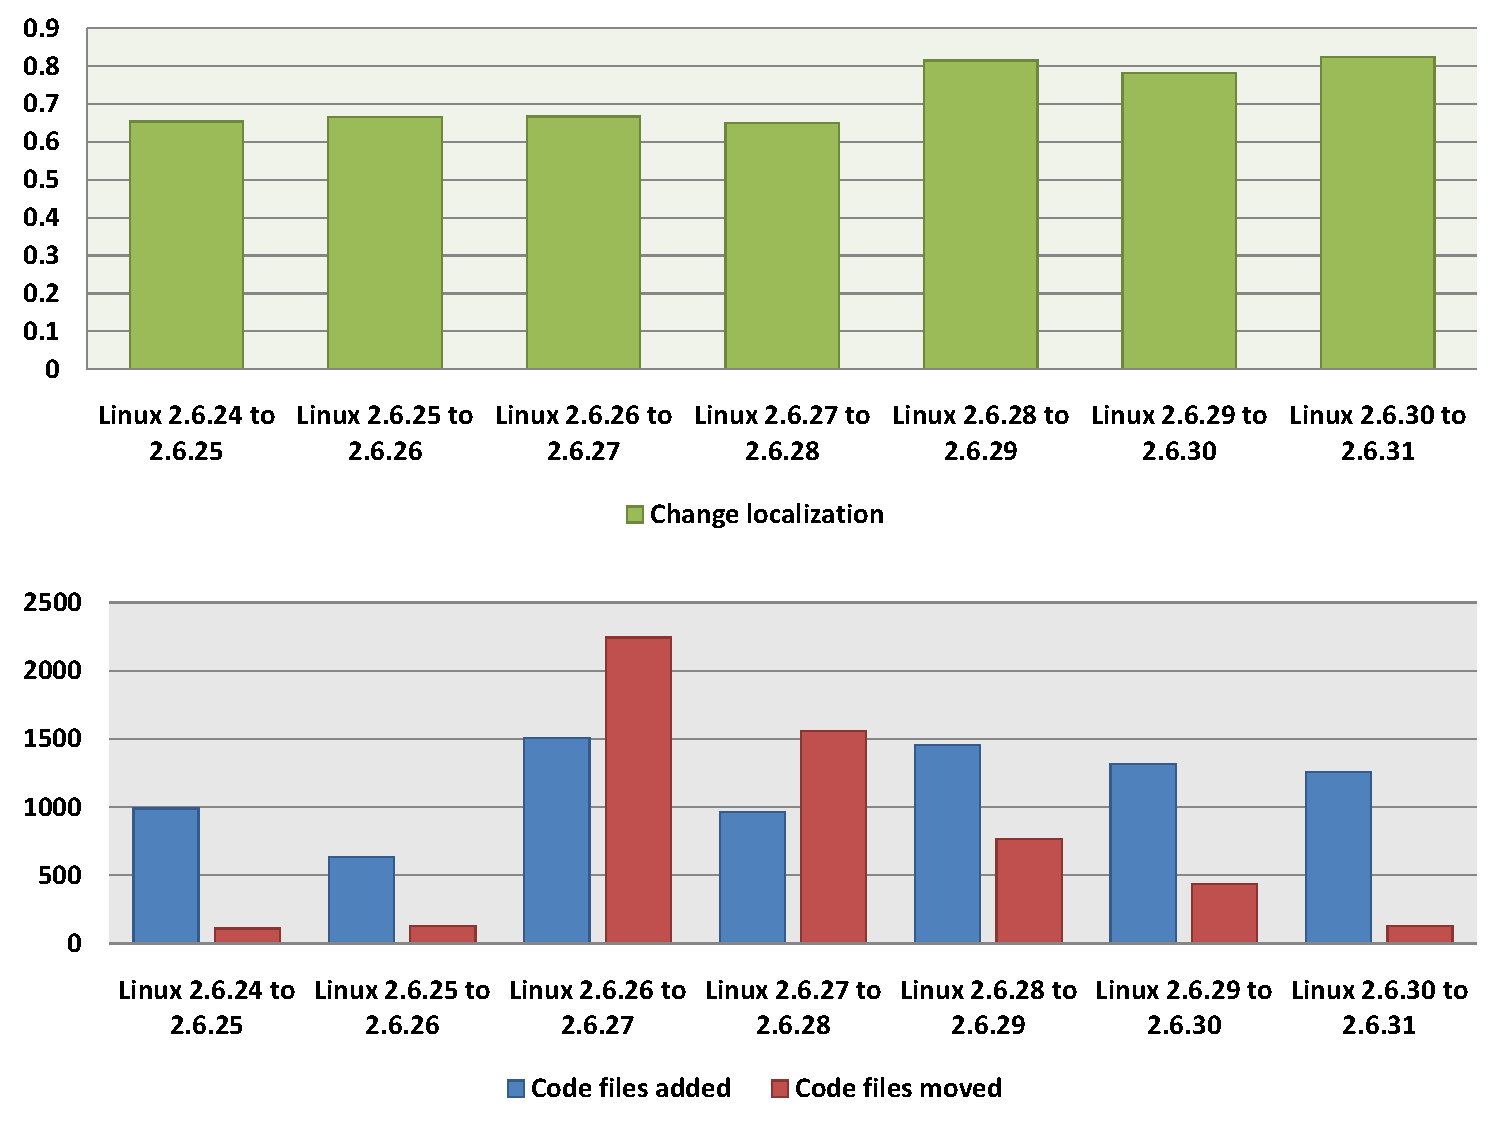
\includegraphics[width=0.95\textwidth]{minings/linux-2-6-fis-metrics}
  \end{center}
\end{frame}

\note{
}

\subsection{Wine}

\begin{frame}{Wine}
  \begin{columns}[c]
    \begin{column}{0.70\textwidth}
      \begin{itemize}
      \item Allows execution of Microsoft Windows programs on
        Unix-like operating systems
      \item Repository checked out on November 20, 2009
      \item $3,479$ code files
      \item $63,864$ commits
      \end{itemize}
    \end{column}
    \begin{column}{0.30\textwidth}
      
\includegraphics[width=\textwidth]{figures/wine-logo}
    \end{column}
  \end{columns}
\end{frame}

\note{
}

\begin{frame}{Wine: Frequent Item Set Metrics}
  \begin{center}
    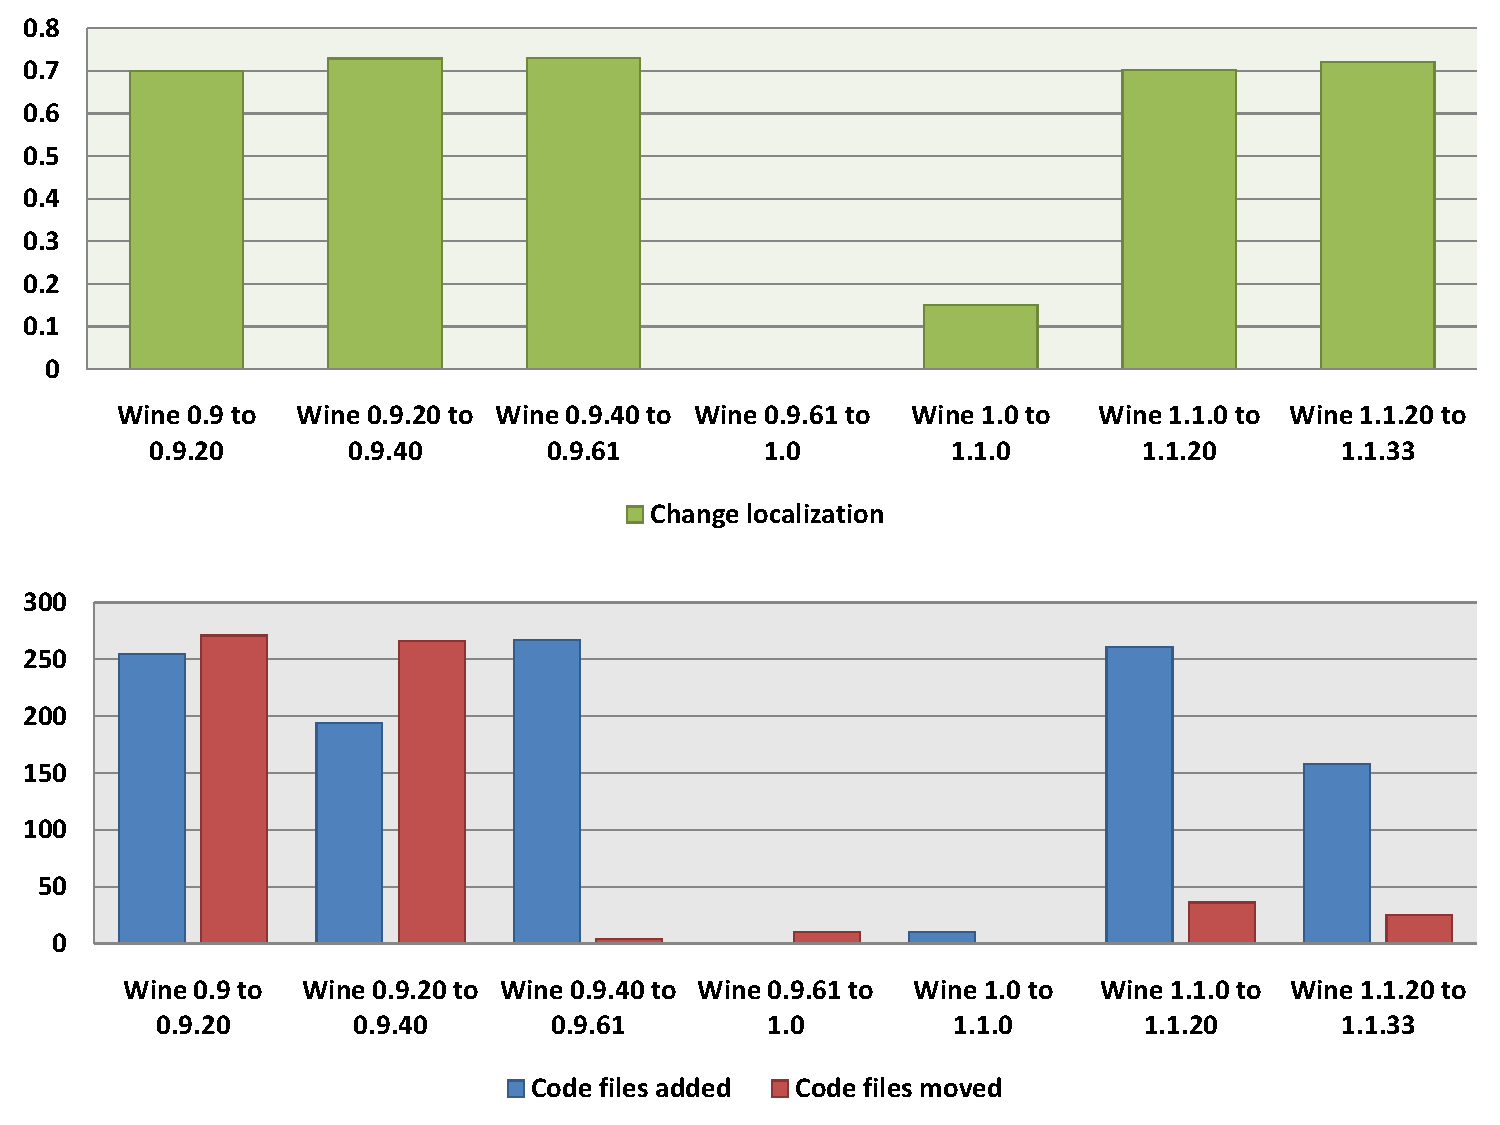
\includegraphics[width=0.95\textwidth]{minings/wine-fis-metrics}
  \end{center}
\end{frame}

\note{
}

\subsection{Insights}

\begin{frame}{Insights}
  \begin{itemize}
  \item Code file moves increase localization
  \item Adding of many code files decrease localization
  \item Adding of code files can clear effect of moves on localization
  \item Stable versions contain mostly bug fixes \\
    $\text{ }\Rightarrow$ low localization, only few moves and adds
  \item Unstable versions contain mostly new features \\
    $\text{ }\Rightarrow$ high localization, many moves and adds
  \end{itemize}
\end{frame}

\note{
}


\section*{Outro}

\begin{frame}{Future Work}
  \begin{itemize}
  \item Use framework to mine software repositories of commercial
    systems
  \item Compare localization metrics of Open Source and Closed Source
    systems
  \item Use the frequent item sets extracted to come up with a better
    modularization
  \item Publish research in the form of a paper
  \end{itemize}
\end{frame}

\note{
}

\begin{frame}{Summary}
  \begin{itemize}
  \item Mining software repositories for intelligent
    software maintenance
  \item Applications of frequent item set mining in improving software
    maintainability
  \item Framework for preventing software maintenance
  \item New metrics for change localization
  \item Localization of frequent item sets of Open Source projects
  \end{itemize}

  \vspace{\stretch{1}}

  \begin{center}
    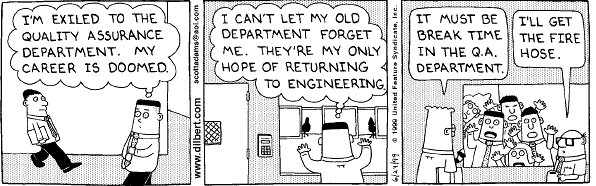
\includegraphics[width=0.7\textwidth]{figures/dilbert-quality-assurance}
  \end{center}
\end{frame}

\note{
  \begin{itemize}
  \item Presented mining software repositories for intelligent
    software maintenance
  \item Shown applications of frequent item set mining in improving
    software maintainability
  \item Implemented framework for preventing software maintenance
  \item Introduced new metrics for change localization
  \item Measured and analyzed localization of frequent item sets of
    Open Source projects
  \end{itemize}
}

\end{document}
